%\negspacechap
\chapter{RESULTADOS Y ANÁLISIS}
	\negspacesec
	%\section{Métricas de error}
\section{RENDIMIENTO DE LOS MÓDULOS} \label{metricas-error}
Al entrenar las redes neuronales, se siguió el procedimiento estándar de separar el conjunto de datos en entrenamiento y validación cruzada para analizar si el modelo está aprendiendo o memorizando los datos.

Así se seleccionan los parámetros de las iteraciones o epochs con menor error en el conjunto de validación cruzada, detallados en la tabla \ref{accuracies}, cuyas gráficas (figuras \ref{drivenetcurve}, \ref{depthnetcurve} y \ref{semsegnetcurve}) fueron descritas en la sección 3.5.

\begin{center}
	\footnotesize
	\begin{tabular}{|c|c|c|}
		\hline
		\textbf{Modelo} & \textbf{Error cuadrático medio} & \textbf{Iteración}\\
		\hline
		DriveNet & 0.00088 & 24\\
		\hline
		DepthNet & 9.267 & 20\\
		\hline
		SemsegNet & 0.09178 & 7\\
		\hline
	\end{tabular}
	\captionof{table}{Errores en el conjunto de validación de los parámetros seleccionados}\label{accuracies}
\end{center}

\subsection{ACELERACIÓN Y GIRO}
	Debido a que el error cuadrático medio penaliza de manera ponderada los valores más lejanos por sobre los cercanos, razón por la cual es una buena métrica de error a la hora de ajustar modelos, es difícil darle una interpretación comprensible al reportar resultados, es por eso que se calcula el error absoluto medio de las predicciones con los valores reales esperados del conjunto de validación.
	
	Para el caso de la predicción de aceleración, considerando que las redes no predicen el uso de frenos sino que estos se aplican cuando el modelo reacciona a semáforos u objetos cercanos, se obtiene un error absoluto medio de 0.067, es decir que la predicción de aceleración oscila $\pm 0.067$ de su valor real, esto debido a que la aceleración no es muy variable en el conjunto de datos de entrenamiento, por lo que al haber pocas situaciones inesperadas, las predicción es un número fijo con pocas variaciones en curvas.
	
	De manera similar para la dirección suavizada por la media exponencial móvil, se obtiene un error de $\pm 0.069$. Este error es mayor al de la aceleración, debido a que es más complicado para las redes mantener una dirección estable si no tiene información temporal, a pesar del uso de medias móviles exponenciales, esta no puede compensar todos los casos de variación.
	
	\begin{figure}[H]
		\centering
		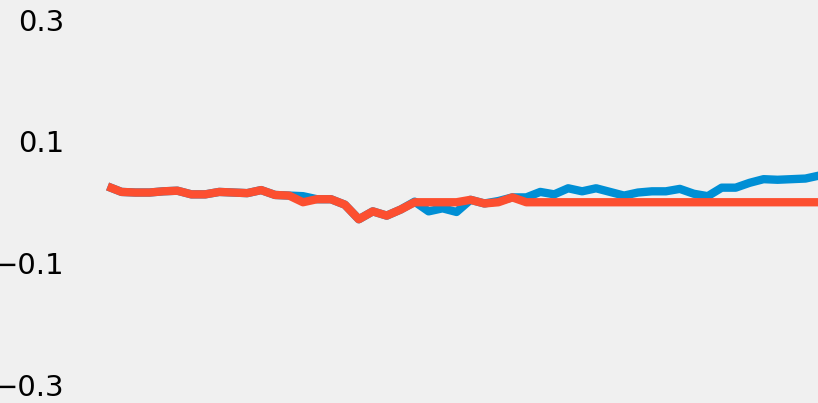
\includegraphics[scale=0.3]{imagenes/preds/ema}
		\caption[Predicción Media Móvil Exponencial]{media móvil exponencial (rojo) suavizando los giros originales (azul)}
		\label{emapred}
	\end{figure}
	
	A pesar de las diferencias calculadas, el error es lo suficientemente pequeño para que no existan acelerones inesperados o giros que causen desestabilidad al vehículo, por lo que se consideraran errores aceptables en la práctica.
	
\subsection{ESTIMACIÓN DE PROFUNDIDAD}
	Al ser también una tarea de predicción de valores en $\mathbb{R}$, se calcula el error absoluto medio entre el mapa de profundidades estimado por la red y el del conjunto de datos de validación.
	
	En este caso el error es de $\pm 1.1931$, el cual es mucho más elevado que los errores de la red de conducción, esto debido a que las posibilidades de error son mayores ya que se predice la distancia pixel a pixel.

	La consecuencia de esto se nota mayormente al encontrarse con objetos cercanos, donde se puede predecir erróneamente que está muy cerca, en cuyo caso el vehículo se detiene totalmente ante un falso obstáculo, o el caso más peligroso que se da cuando el objeto está muy cerca y se predice que está una unidad más lejos del límite en el cual el modelo decide detener el auto y se produce una colisión.
	
	Gráficamente en la figura \ref{depthpred} se observa que la predicción es ``borrosa'' comparado con el mapa de profundidad original.
	
	\begin{figure}[H]
		\centering
		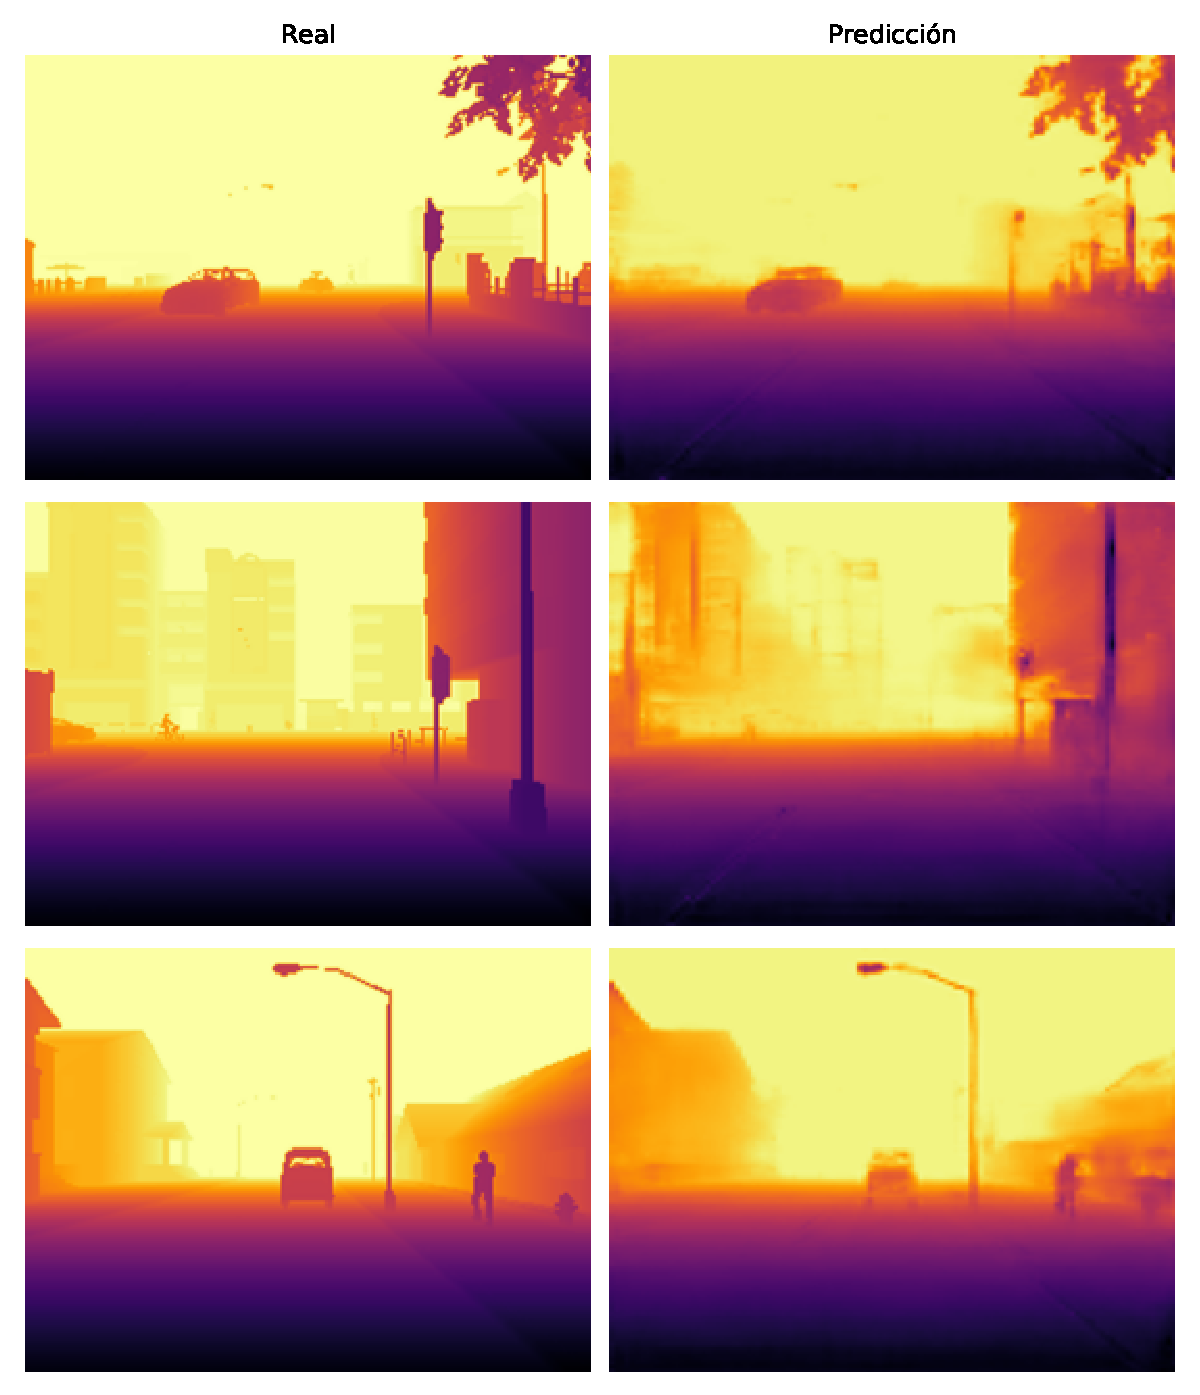
\includegraphics[scale=0.6]{imagenes/preds/depth}
		\caption[Predicción vs valor esperado de profundidad]{predicción vs valor esperado de profundidad}
		\label{depthpred}
	\end{figure}
	
\subsection{SEGMENTACIÓN SEMÁNTICA}
El módulo de segmentación semántica, considerando la limpieza de predicciones residuales mediante erosión, dilatación y apertura, es uno de los componentes más importantes, ya que la detención ante obstáculos y la detección de objetos depende de las predicciones de esta red, además, al ser una tarea de clasificación, se pueden analizar los resultados a mayor detalle con distintas métricas de error.
	\subsubsection{MATRIZ DE CONFUSIÓN}
	Se realiza el cálculo de la matriz de confusión, sin embargo, al existir muchas ocurrencias de cada clase, se decide estandarizar los valores a porcentajes por fila para mejor visualización, teniendo así la figura \ref{confussionmat}, dónde las diagonales indican los valores predichos correctamente, y fuera de la diagonal están las detecciones erróneas.
	
	\begin{figure}[H]
		\centering
		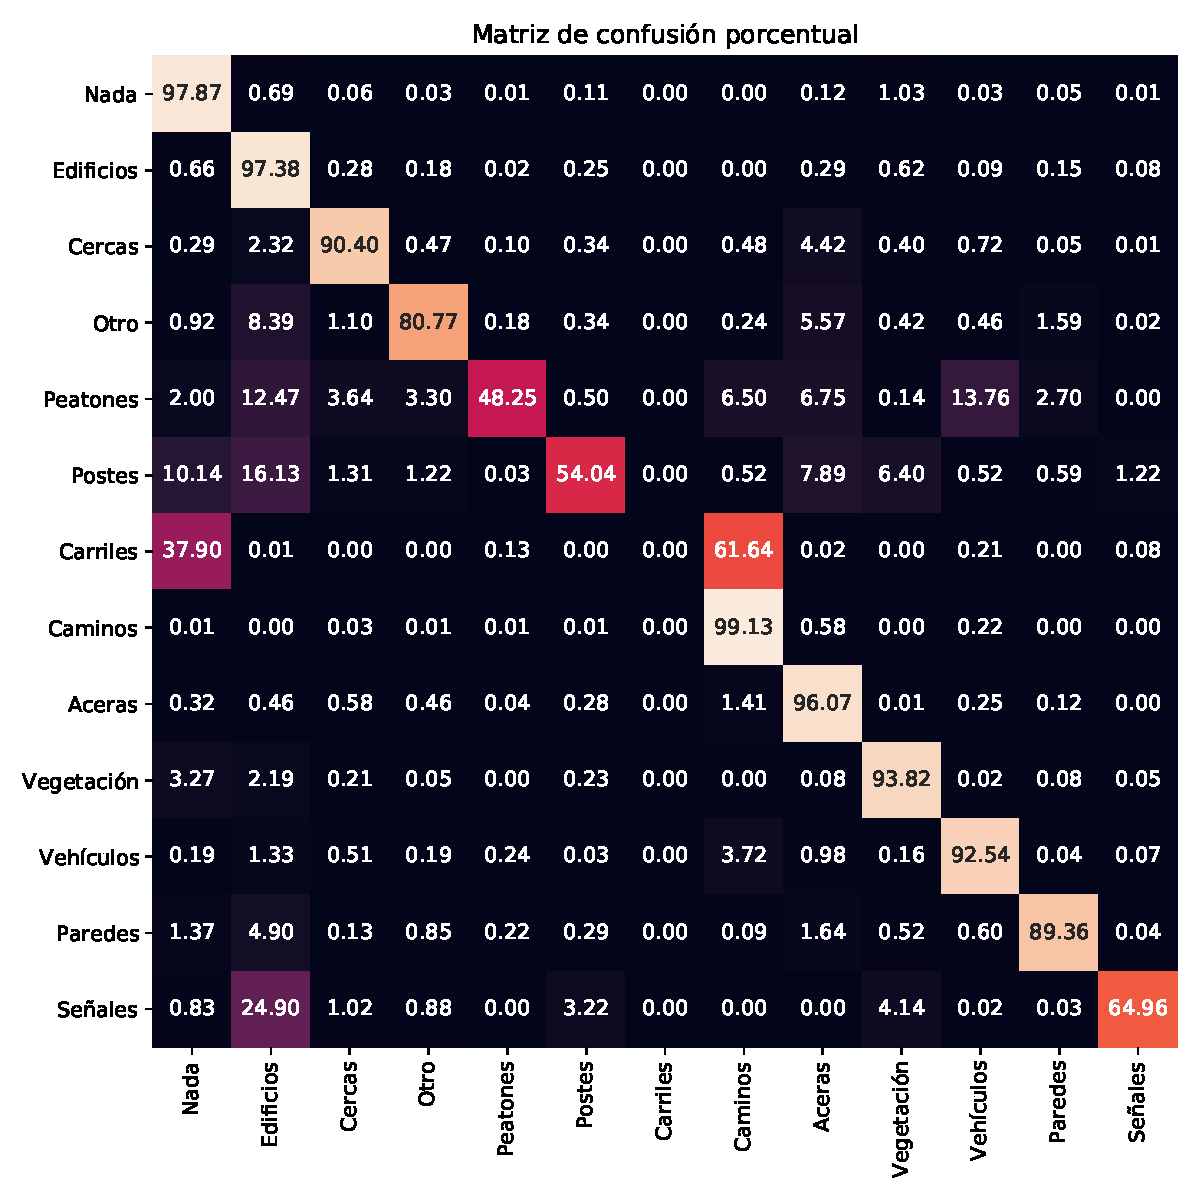
\includegraphics[scale=0.6]{imagenes/c_mat}
		\caption[Matriz de confusión de segmentación semántica]{matriz de confusión de segmentación semántica}
		\label{confussionmat}
	\end{figure}

	Se puede observar en la figura \ref{confussionmat}, que cuatro clases que se utilizan en la conducción, las cuales son peatones, postes, vehículos y señales de tránsito, tienen porcentajes de predicción de verdaderos positivos $48.25\%$, $54.04\%$, $92.54\%$ y $64.96\%$ respectivamente, siendo la detección de peatones y postes la menos exacta, la primera porque los peatones normalmente aparecen en aceras y en los bordes del campo de visión, y los postes debido a que son delgados y por la baja resolución de predicción es difícil para la red segmentarlos completamente.
	
	\subsubsection{PRECISIÓN Y EXHAUSTIVIDAD}
	Una vez se tiene la matriz de confusión, se pueden calcular la exactitud pixel a pixel, precisión, exhaustividad y el valor-F por clases, los cuales se listan en la tabla \ref{metricas}
	
%	Precision: Del total clasificado correctamente, cuánto porciento de estos son positivos.
%   Recall: Del total de los positivos, cuanto porciento son clasificados como positivos
	\begin{center}
		\footnotesize
		\begin{tabular}{|c|c|c|c|}
			\hline
			\textbf{Clase} & \textbf{Precisión} & \textbf{Exhaustividad} & \textbf{Valor-F}\\
			\hline
			Edificios  & 0.963 & 0.9738 & 0.9684\\
			\hline
			Cercas     & 0.8929 & 0.904 & 0.8984\\
			\hline
			Peatones   & 0.7141 & 0.4825 & 0.5759\\
			\hline
			Postes     & 0.7398 & 0.5404 & 0.6246\\
			\hline
			Carriles   & 0.0 & 0.0 & 0.0\\
			\hline
			Caminos    & 0.9855 & 0.9913 & 0.9884\\
			\hline
			Aceras     & 0.9517 & 0.9607 & 0.9562\\
			\hline
			Vegetación & 0.9218 & 0.9382 & 0.9299\\
			\hline
			Vehículos  & 0.9402 & 0.9254 & 0.9327\\
			\hline
			Paredes    & 0.8707 & 0.8936 & 0.882\\
			\hline
			Señales    & 0.7802 & 0.6496 & 0.7089\\
			\hline
		\end{tabular}
		\captionof{table}[Métricas de error de clasificación]{métricas de error de clasificación}\label{metricas}
	\end{center}

	De la tabla de errores y la matriz de confusión se puede notar primeramente que debido al desbalance de las muestras por clase, las predicciones de líneas de carriles son todas negativas, lo cual da una idea engañosa de alta exactitud, sin embargo el valor F, usado para compensar este sesgo dejan en claro que en realidad la predicción es totalmente errónea. Esto no es un problema para el modelo debido a que no se usa esta clase para las predicciones.
	
	Para las cuatro clases utilizadas tenemos que:
	\begin{itemize}
		\item \textbf{Peatones:} un $71.41\%$ del total de píxeles clasificados correctamente son positivos, $48.25\%$ de positivos reales son clasificados correctamente lo cual indica una alta cantidad de falsos negativos, con una exactitud balanceada de $57.59\%$.
		\item \textbf{Postes:} precisión $73.98\%$ y exhaustividad del $54.04\%$, dando menos falsos negativos con exactitud balanceada de $62.46\%$.
		\item \textbf{Vehículos:} precisión del $94.02\%$, exhaustividad de $92.54\%$ y exactitud de $93.27\%$ siendo esta la clase con los menores errores de predicción.
		\item \textbf{Señales de tránsito:} precisión $78.02\%$, exhaustividad $64.96\%$, con muchos menos falsos negativos, y $70.89\%$ de exactitud.
	\end{itemize}
	
	\begin{figure}[H]
		\centering
		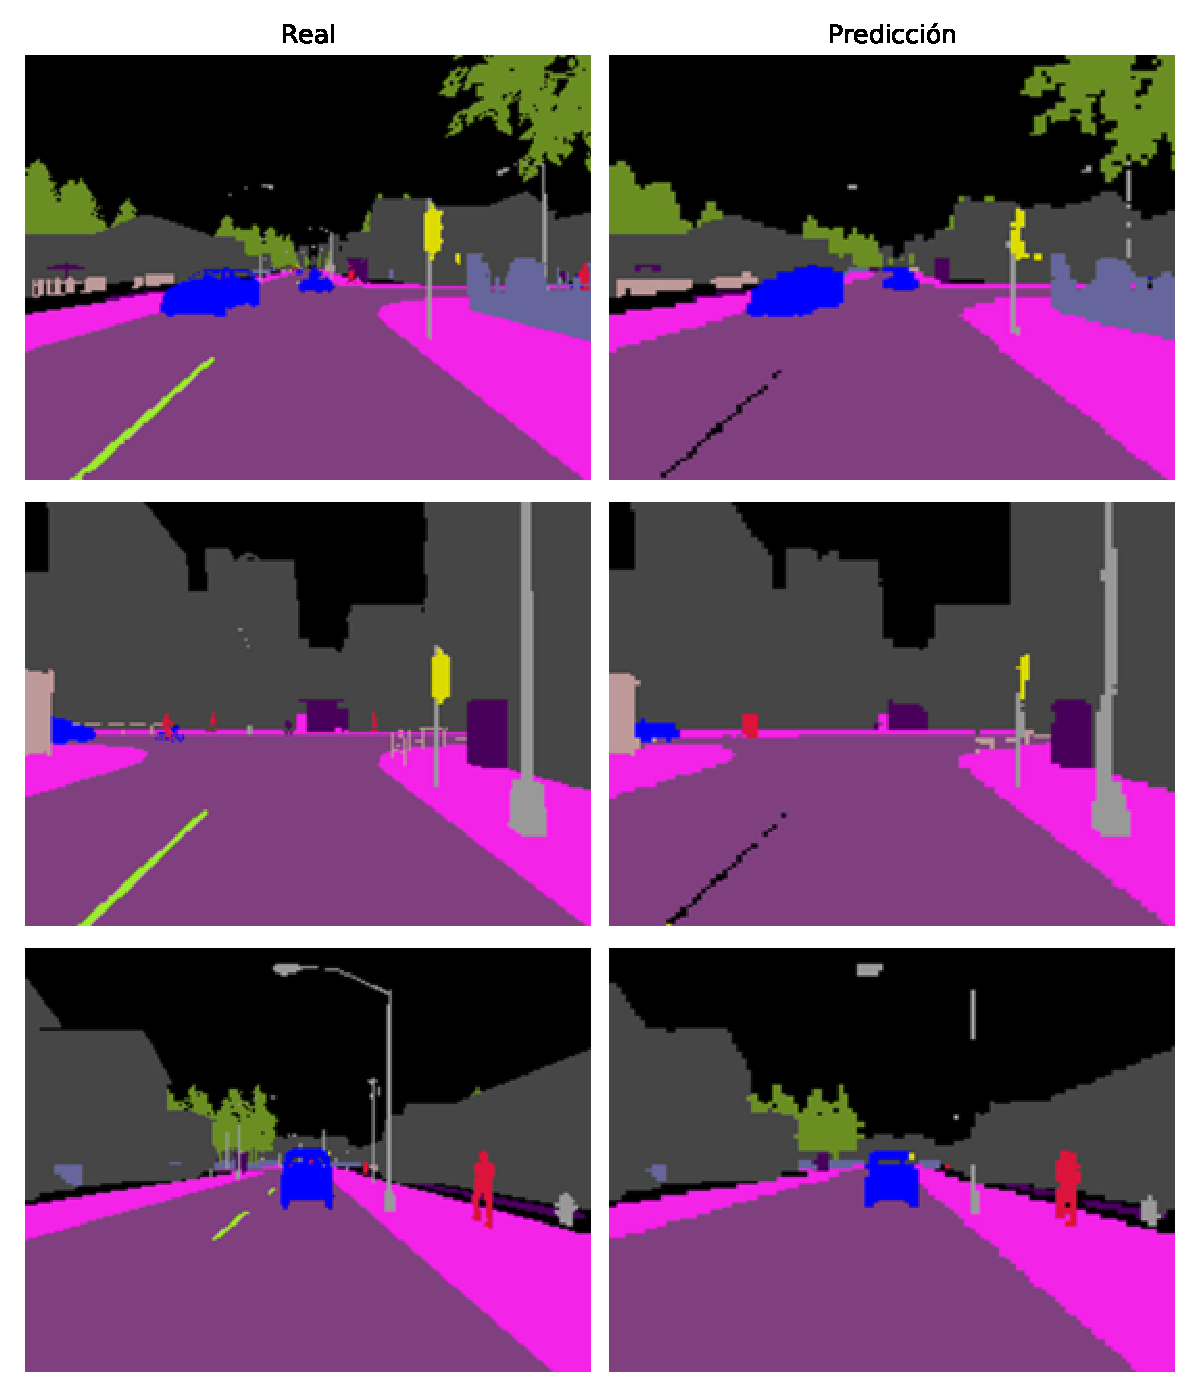
\includegraphics[scale=0.6]{imagenes/preds/semseg}
		\caption[Predicción vs valor esperado de segmentación]{predicción vs valor esperado de segmentación}
		\label{semsegpred}
	\end{figure}
	
	Por estos resultados se puede afirmar que la detección de vehículos es la más exacta dando lugar a muy pocos casos en que no se los detecte para una parada efectiva. Por otra parte al detectar Peatones, Postes y Señales de tránsito en general, se tiene alta exhaustividad, es decir que si bien se detecta una cantidad considerable de píxeles de la clase, tiende a detectar menos píxeles de los que realmente componen al objeto (como se observa en la figura \ref{semsegpred}), sin embargo debido a la alta precisión, estos píxeles detectados tienen una alta confianza de ser de la clase predicha, en otras palabras, el modelo discrimina de manera agresiva, de forma que pocos valores pasan el umbral de clasificación, pero los que pasan tienen más seguridad de ser correctos.
	
	Una de las consecuencias de la alta exhaustividad, que se detallará en las pruebas del simulador, es que pueden no detectarse postes a tiempo dando lugar a colisiones.
	
	\subsubsection{CAJAS DELIMITADORAS}
	Finalmente, haciendo uso de las máscaras de segmentación por clase, se pueden visualizar las cajas delimitadoras de los objetos, haciendo uso del flood fill, para comprobar las predicciones gráficamente mediante un código de color para cada clase, celeste para vehículos, naranja para peatones, rosado para postes y rojo o verde para semáforos dependiendo de su estado.
	
	\begin{figure}[H]
		\centering
		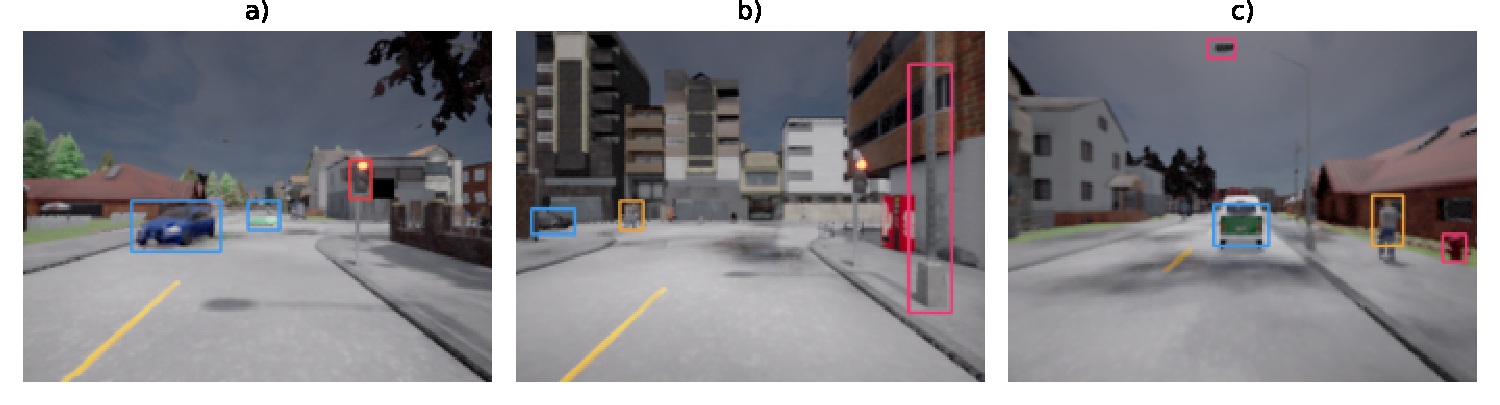
\includegraphics[scale=0.64]{imagenes/preds/boxes}
		\caption[Cajas delimitadoras]{cajas delimitadoras}
		\label{boxes}
	\end{figure}

	en el caso de la figura \ref{boxes}, se observa que en la imagen b, no se detectó el semáforo, debido a que el área de la segmentación es muy pequeña para ser considerada una clasificación válida, de manera similar en la imagen c, sólo se detecta la parte de la luz del poste.
	
	\subsubsection{ÍNDICE JACCARD}
	Aplicando el índice de Jaccard, conocido como Intersection Over Union (IoU), otra métrica útil en la segmentación semántica, se obtiene la siguiente tabla de porcentajes:
	
	\begin{center}
		\footnotesize
		\begin{tabular}{|c|c|}
			\hline
			\textbf{Clase} & \textbf{IoU}\\
			\hline
			Edificios & 90.88\%\\
			\hline
			Cercas &  69.54\%\\
			\hline
			Peatones & 45.72\%\\
			\hline
			Postes & 31.93\%\\
			\hline
			Carriles & 03.52\%\\
			\hline
			Caminos & 97.55\%\\
			\hline
			Aceras & 91.01\%\\
			\hline
			Vegetación & 77.76\%\\
			\hline
			Vehículos & 72.46\%\\
			\hline
			Paredes & 57.26\%\\
			\hline
			Señales & 37.25\%\\
			\hline
		\end{tabular}
		\captionof{table}[Índice de Jaccard]{Índice de Jaccard de la segmentación semántica}\label{iou}
	\end{center}

	si se interpretan los valores como el porcentaje de superposición de la máscara real y la máscara predicha para cada clase, se observa que de las cuatro clases que más nos interesan los postes y señales de tránsito tienen los peores valores debido a la alta discriminación de píxeles de la red neuronal, mientras que los peatones y vehículos tienen mayor porcentaje, útil para evadirlos como obstáculos en la vía.
	
\subsection{DETECCIÓN Y CLASIFICACIÓN DE SEMÁFOROS}
	% Porcentaje de semáforos correctamente clasificados
	Debido a que el segmentador no discierne entre semáforos y las demás señales de tránsito, la clasificación de si lo es o no, y su color depende del módulo basado en K-means, evaluando la exactitud de este componente, se obtuvo que clasifica correctamente semáforos verdes en un $98.65\%$ de entre $1848$ pruebas, y rojos en un $99.52\%$ de exactitud de $2102$ imágenes. El $1.35\%$ de error en el color verde se da cuando se clasifican erroneamente semáforos amarillos que para la tarea se consideran igual a los rojos. Por otra parte el $0.48\%$ de error en semáforos rojo se debe al porcentaje de falsos negativos, es decir, la proporción de rojos reales clasificados como otro tipo de señal de tránsito. Así la exactitud total de clasificación de los colores es de $99.08\%$.
	
	\begin{figure}[H]
		\centering
%		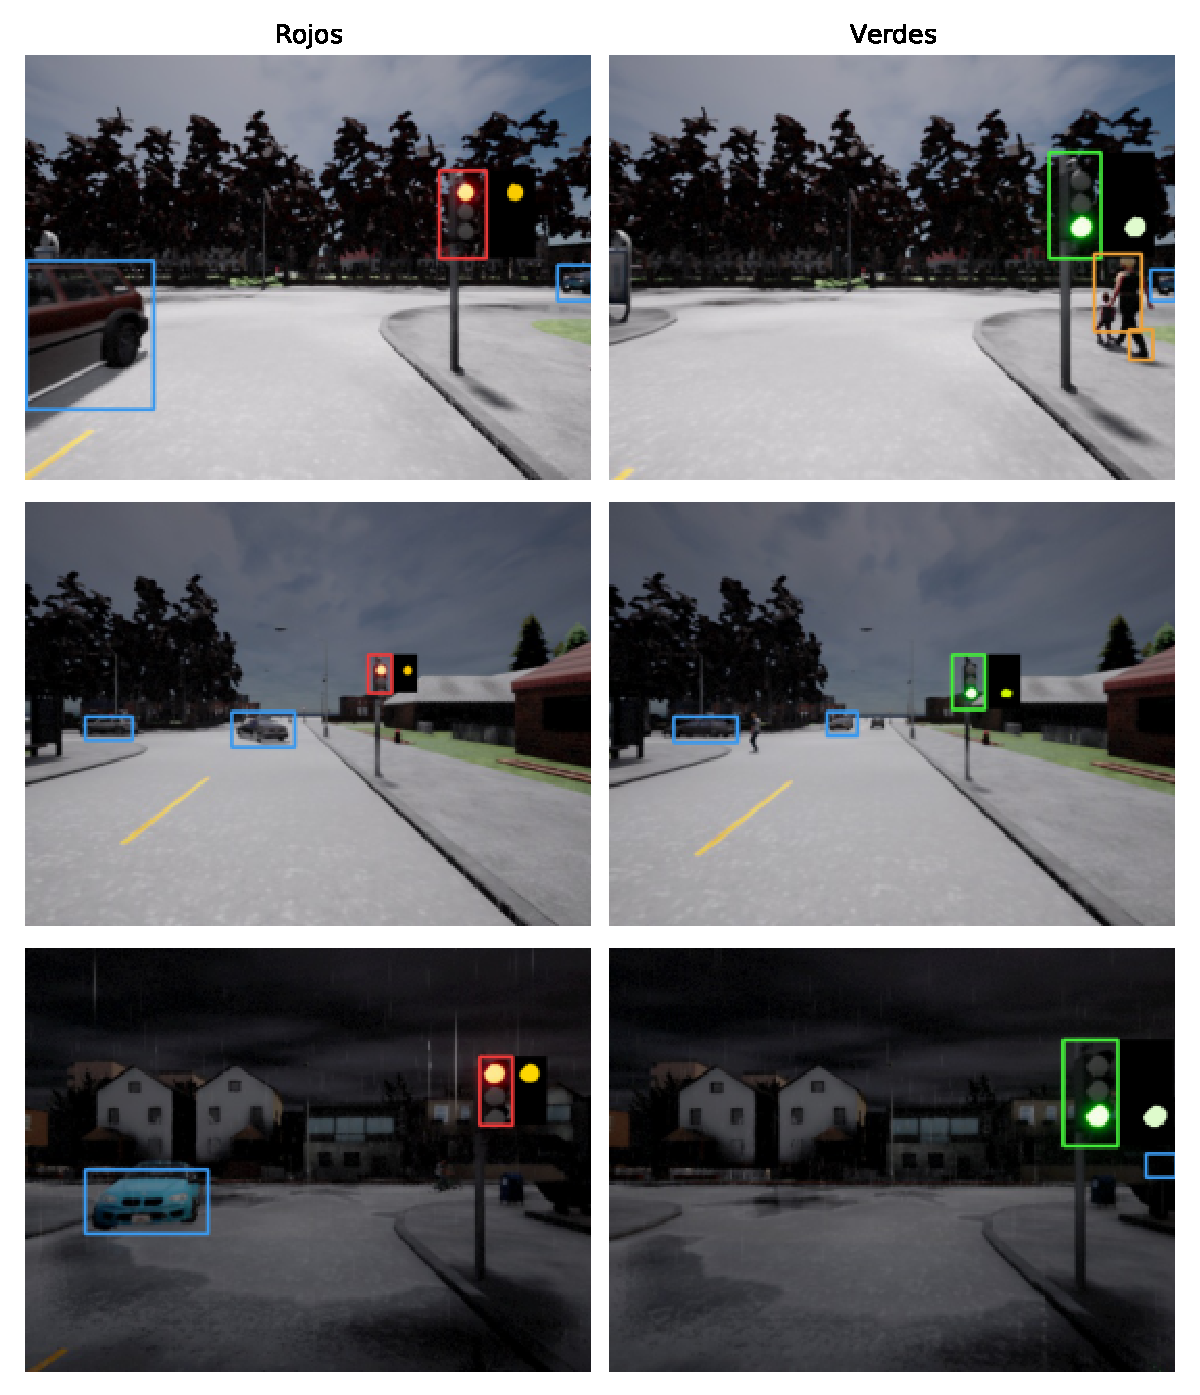
\includegraphics[scale=0.65]{imagenes/preds/semaforos}
		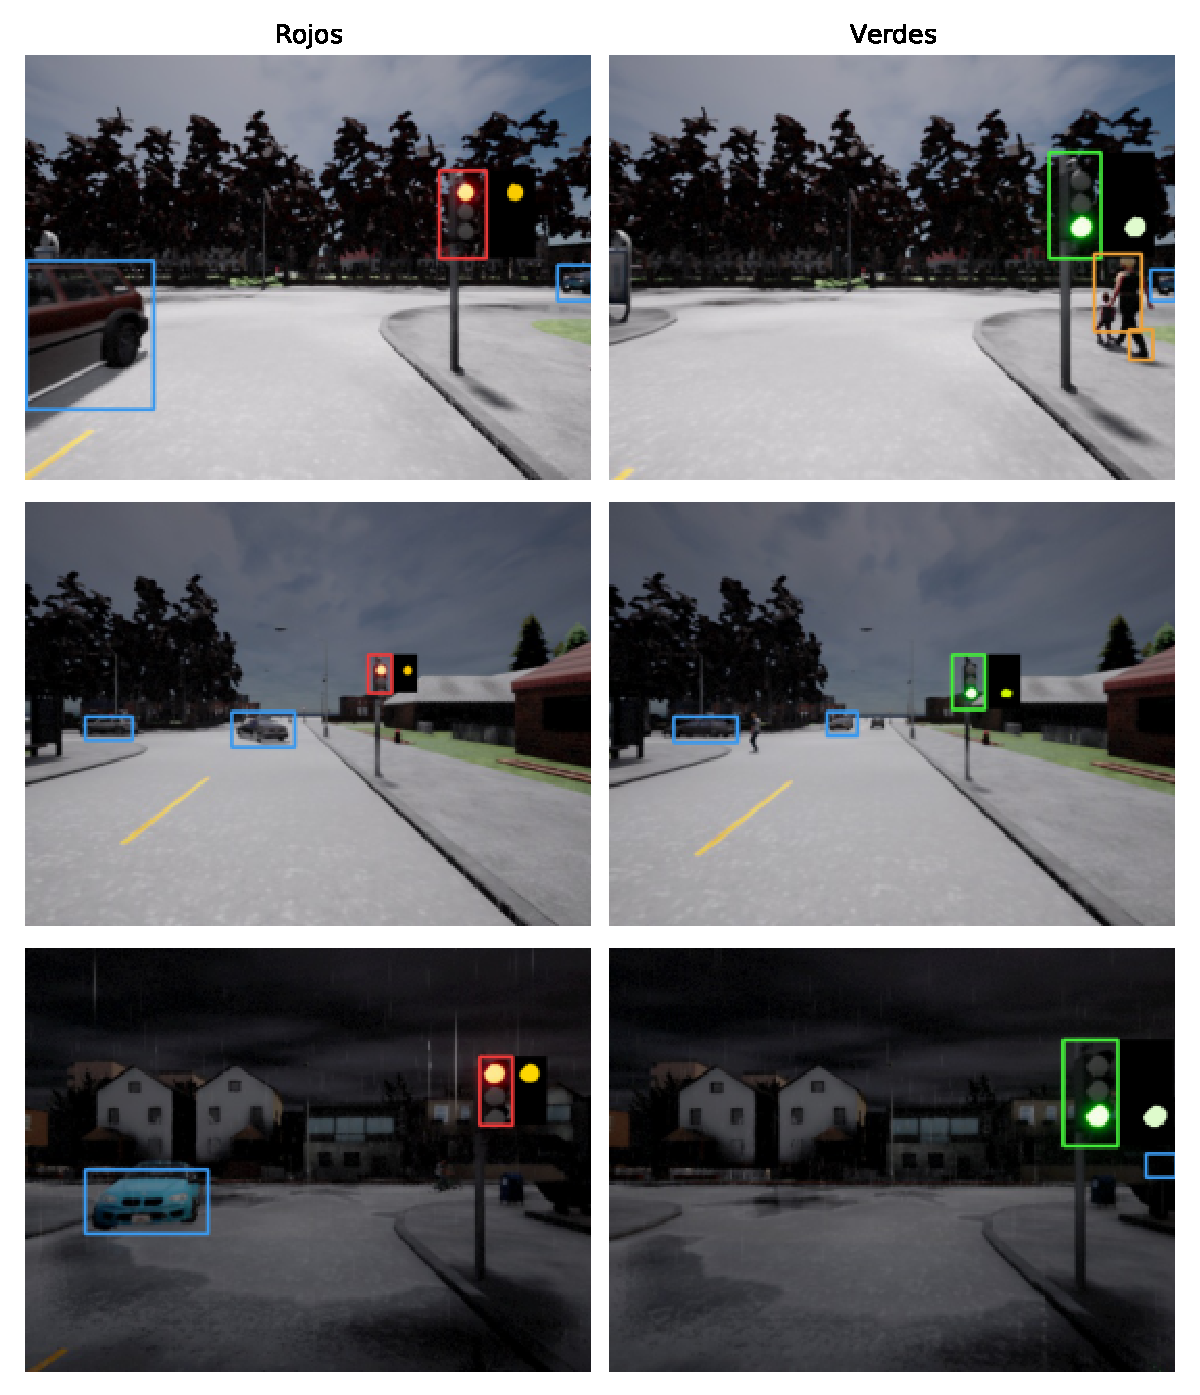
\includegraphics[scale=0.58]{imagenes/preds/semaforos}
		\caption[Cuantización y Clasificación del Color]{cuantización y clasificación del color}
		\label{semaforos}
	\end{figure}
	
	% Semáforos con caja delimitadora
	Una vez calculado el error en la clasificación del color se puede visualizar en la figura \ref{semaforos} las predicciones del módulo. El color de la caja delimitadora indica la predicción, y a su lado se muestra la cuantización realizada por K-Means sobre la que se aplican los umbrales de clasificación.
	
% BACKUP TABLA
%\begin{center}
%	\footnotesize
%	\begin{tabular}{|c|c|c|c|c|}
%		\hline
%		\textbf{Clase} & \textbf{Exactitud} & \textbf{Precisión} & \textbf{Exhaustividad} & \textbf{Valor-F}\\
%		\hline
%		Edificios & 0.9874 & 0.963 & 0.9738 & 0.9684\\
%		\hline
%		Cercas    & 0.9963 & 0.8929 & 0.904 & 0.8984\\
%		\hline
%		Peatones  & 0.9991 & 0.7141 & 0.4825 & 0.5759\\
%		\hline
%		Postes    & 0.9951 & 0.7398 & 0.5404 & 0.6246\\
%		\hline
%		Carriles  & 0.9972 & 0.0 & 0.0 & 0.0\\
%		\hline
%		Caminos   & 0.9928 & 0.9855 & 0.9913 & 0.9884\\
%		\hline
%		Aceras    & 0.9907 & 0.9517 & 0.9607 & 0.9562\\
%		\hline
%		Vegetación& 0.9914 & 0.9218 & 0.9382 & 0.9299\\
%		\hline
%		Vehículos & 0.9962 & 0.9402 & 0.9254 & 0.9327\\
%		\hline
%		Paredes   & 0.9984 & 0.8707 & 0.8936 & 0.882\\
%		\hline
%		Señales   & 0.999 & 0.7802 & 0.6496 & 0.7089\\
%		\hline
%	\end{tabular}
%	\captionof{table}[Métricas de error de clasificación]{métricas de error de clasificación}\label{metricas}
%\end{center}
	
	\pospacesec
	\section{REPRESENTACIONES APRENDIDAS} \label{representaciones-aprendidas}
% Distancias en ROI
\subsection{DISTANCIAS EN LA REGIÓN DE INTERÉS}
Al combinar la máscara de segmentación de posibles obstáculos con el mapa de profundidades se simplifica la tarea de calcular la distancia a estos, además al considerar sólo el trapecio delimitando el área de circulación denominada región de interés, se reducen las falsas detecciones, como se puede observar en la figura \ref{distpred}

\begin{figure}[H]
	\centering
	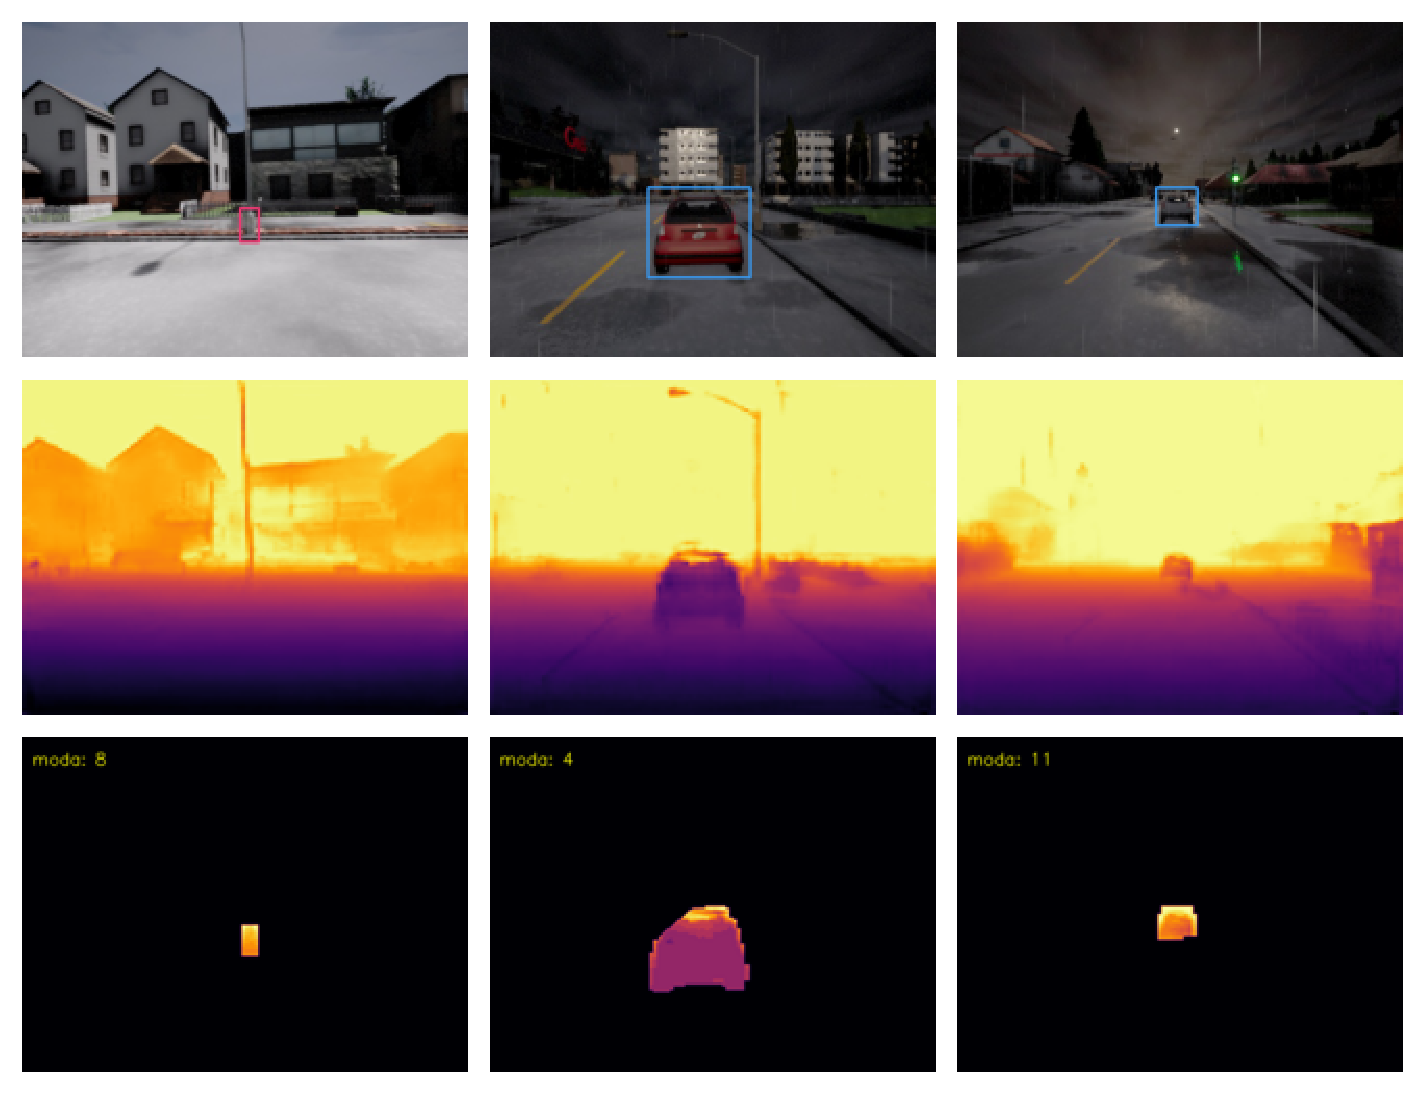
\includegraphics[scale=0.65]{imagenes/preds/distance}
	\caption[Distancia a de objetos]{distancia a objetos en el área de interés}
	\label{distpred}
\end{figure}

en la primera fila se tienen las detecciones generales usando las máscaras de segmentación, en la segunda los mapas de profundidad, y en la tercera la distancia estimada solamente a los posibles obstáculos, esta distancia general se calcula mediante la moda del valor de los píxeles del mapa de profundidades, así en cuanto un objeto está cerca, la mayoría de sus píxeles tendrán un valor bajo, siendo el límite de 4 metros a partir de la cual se empieza a frenar.

\subsection{VISUALIZACIÓN DE ZONAS DE INTERÉS}
% ScoreCam
Con el fin de comprender gráficamente a qué partes de la imagen la red neuronal de conducción presta atención durante la predicción del giro, se aplica el algoritmo scorecam, del cual se obtiene un mapa de calor que une a la imagen original, y cuyos valores altos indican mayor atención en la región.

\begin{figure}[H]
	\centering
	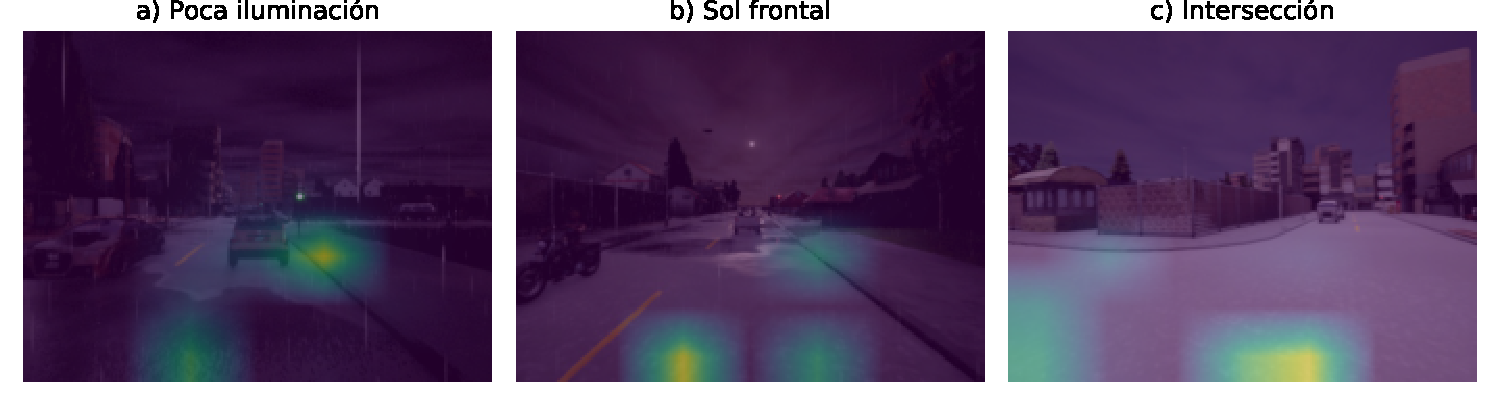
\includegraphics[scale=0.6]{imagenes/preds/scorecam}
	\caption[Regiones de Interés en la Inferencia de Dirección]{regiones de interés en la inferencia de dirección}
	\label{scorecampred}
\end{figure}

En la figura \ref{scorecampred} se observan en los casos $a$ y $b$ que aparte de la atención en el asfalto, debido a que se comparten los filtros para la inferencia de aceleración, se fija en la acera derecha, mientras que en la imagen $c$, al no tener una acera en el lado esperado se centra en la que está al frente, en la nueva calle a incorporarse.
	
	\section{PRUEBAS EN SIMULADOR} \label{pruebas-simulador}
% rendimiento en simulacion (imágenes con giros y sus predicciones),
% gráfica del EMA.
% Casos de predicciones correctas vs erroneas en calles.
% Casos de predicciones correctas vs erroneas en intersecciones.
Una vez se tiene la certeza del funcionamiento del modelo mediante el análisis de sus métricas de error, se comprueban los resultados empíricamente con simulaciones en el ambiente virtual de la ciudad de CARLA.
\subsection{CONDUCCIÓN}
Ya se revisaron los resultados de segmentación, estimación de distancias y clasificación de objetos en la imagen, luego de pasar por todas las etapas descritas del modelo, las salidas obtenidas son el valor del giro y la aceleración.

\begin{figure}[H]
	\centering
	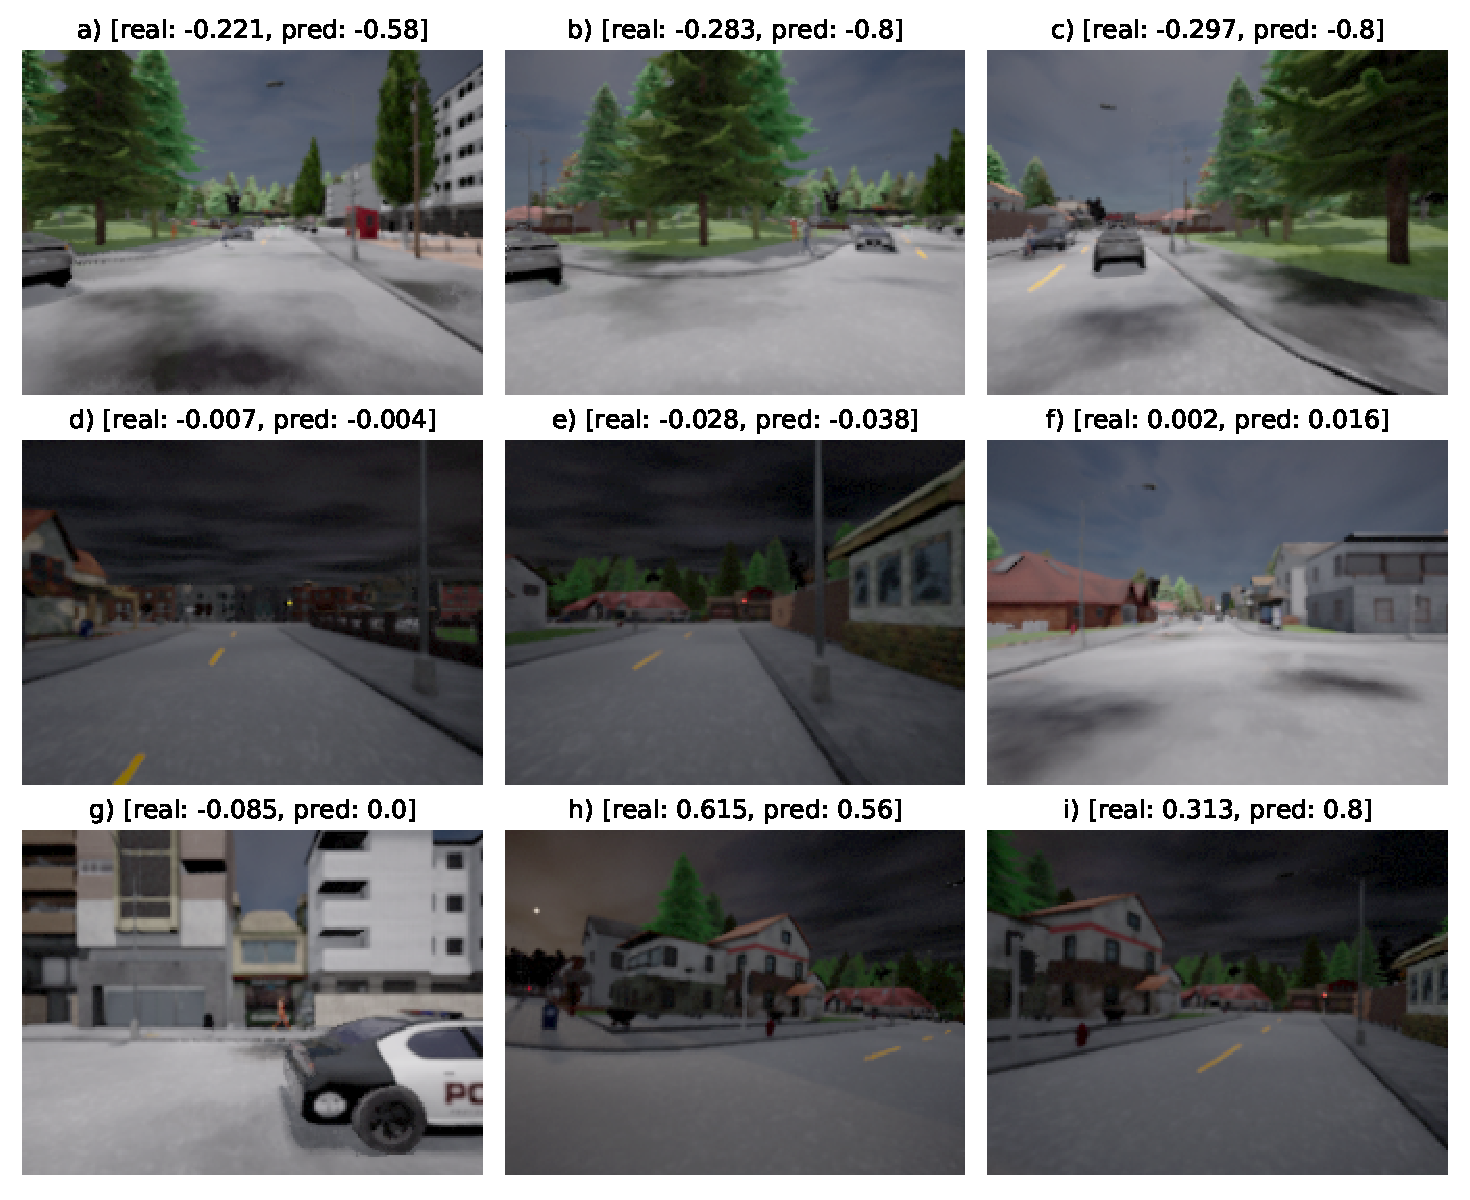
\includegraphics[scale=0.63]{imagenes/preds/steer}
	\caption[Comparación de Dirección Real y Estimada]{comparación de dirección real y estimada}
	\label{steer}
\end{figure}

Comparando las predicciones en distintas situaciones se tienen los resultados de la figura \ref{steer}, de la cual se puede observar en los casos $a, b, c, h, i$, los cuales consisten en giros durante intersecciones, que el modelo es mucho más agresivo al tomar las curvas, aplicando un giro mayor de la dirección. En el caso $f$ que es una intersección en la cual se decide seguir recto, predice correctamente no girar. En la situación de la imagen $g$, se tiene una casi colisión con otro vehículo, en cuyo caso la predicción es 0, al igual que la aceleración, y finalmente en las imágenes $d$ y $e$ no existe mucha variación del $0$ ya que se encuentra en una recta dentro de su carril.

\subsection{FALLOS}
A pesar del buen rendimiento del modelo en las situaciones de prueba, siempre existe un margen de error contemplado en las métricas evaluadas, así se presentan situaciones puntuales donde el vehículo se detiene abruptamente al confundir charcos de agua en la vía con vehículos cercanos (figura \ref{charco}), o los más graves cuando se sale del camino y colisiona con objetos en las aceras \ref{colision}.

\begin{figure}[H]
	\centering
	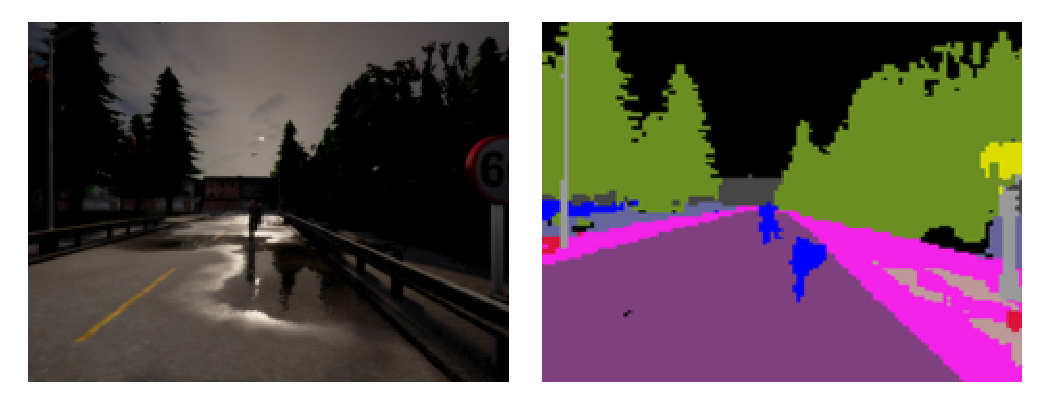
\includegraphics[scale=0.7]{imagenes/preds/err1}
	\caption[Charco erroneamente Clasificado]{Charco erroneamente Clasificado}
	\label{charco}
\end{figure}

%\begin{figure}[H]
%	\centering
%	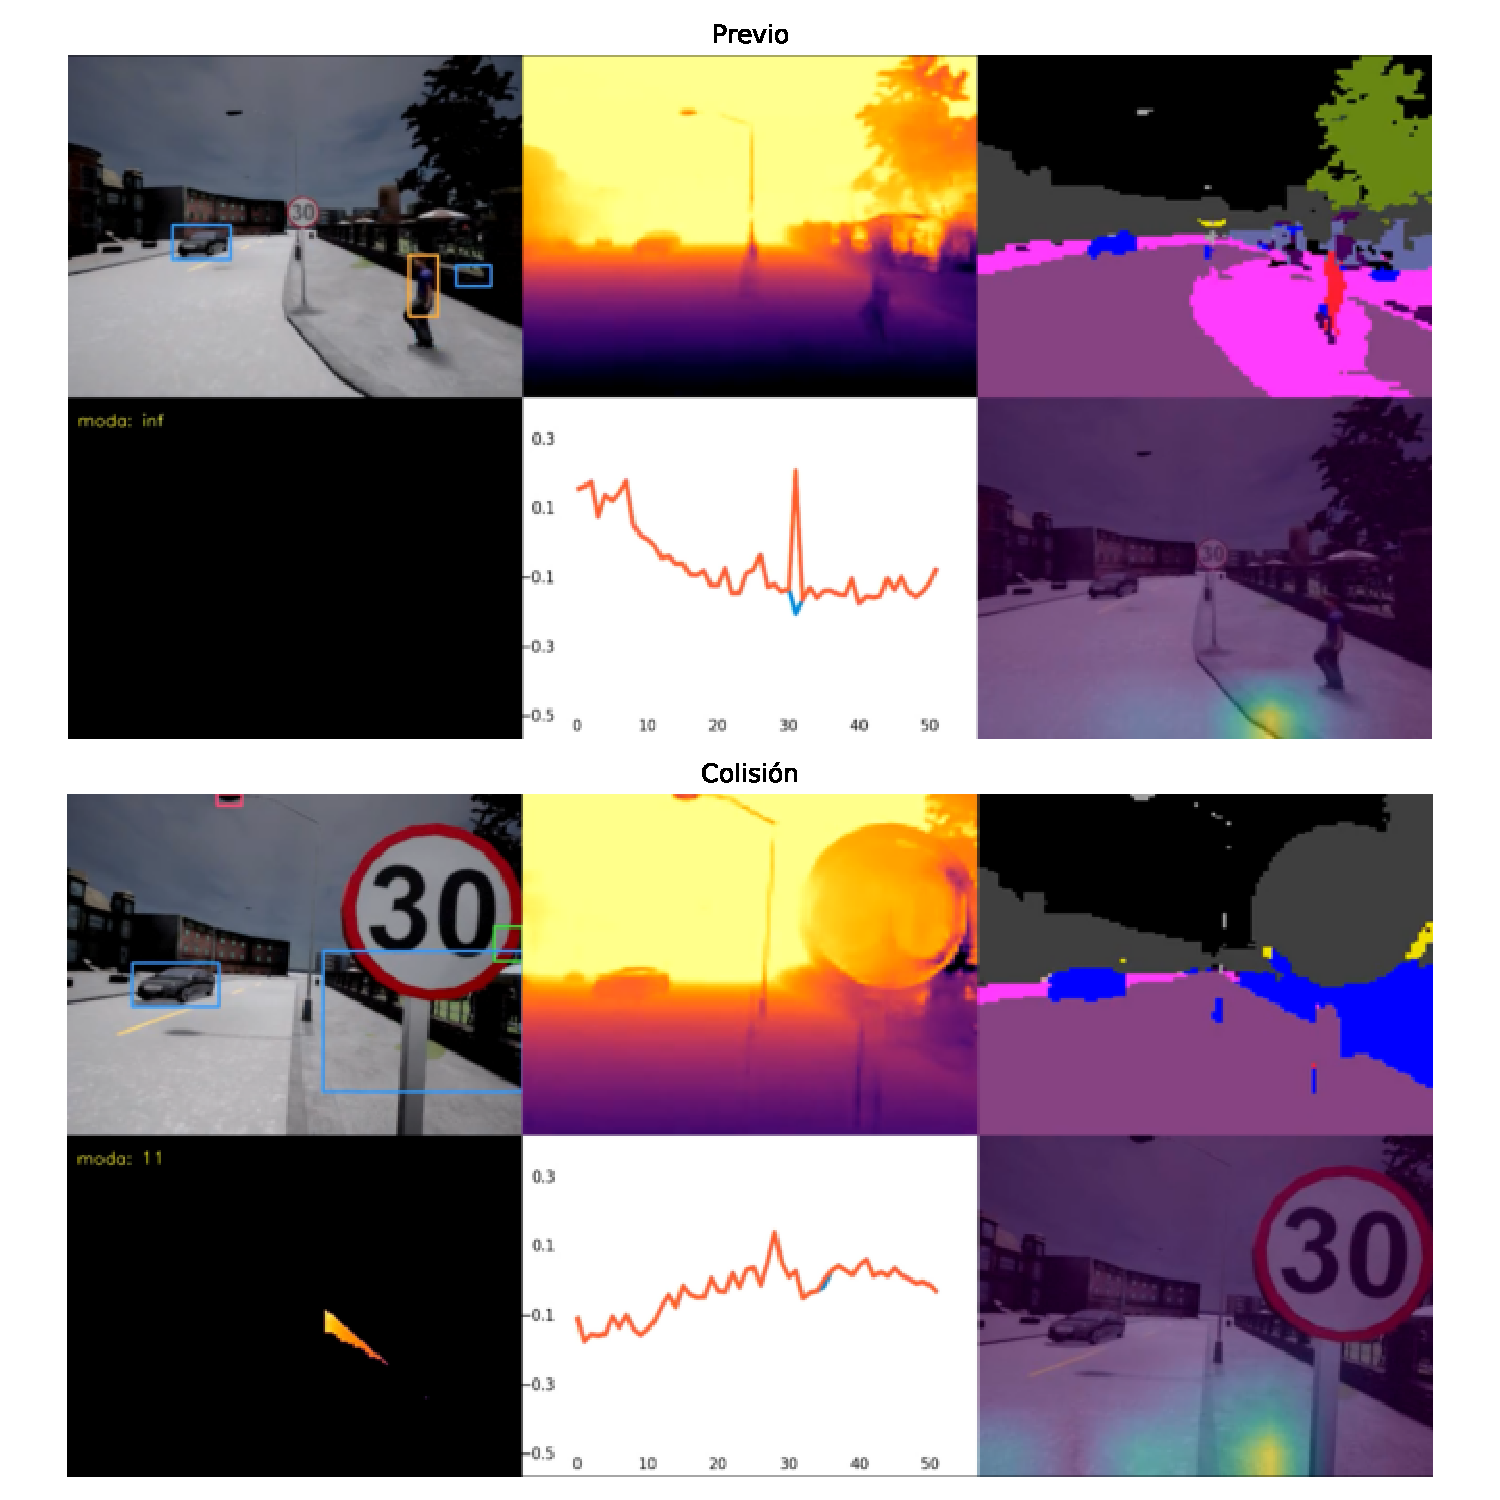
\includegraphics[scale=0.6]{imagenes/preds/err2}
%	\caption[Colisión con Poste]{colisión con poste}
%	\label{colision}
%\end{figure}

En la figura \ref{colision} se nota que la segmentación falla al no detectar el poste como obstáculo lo cual deriva en que no se calcule la distancia a este y se produzca la colisión.

\begin{figure}[H]
	\centering
	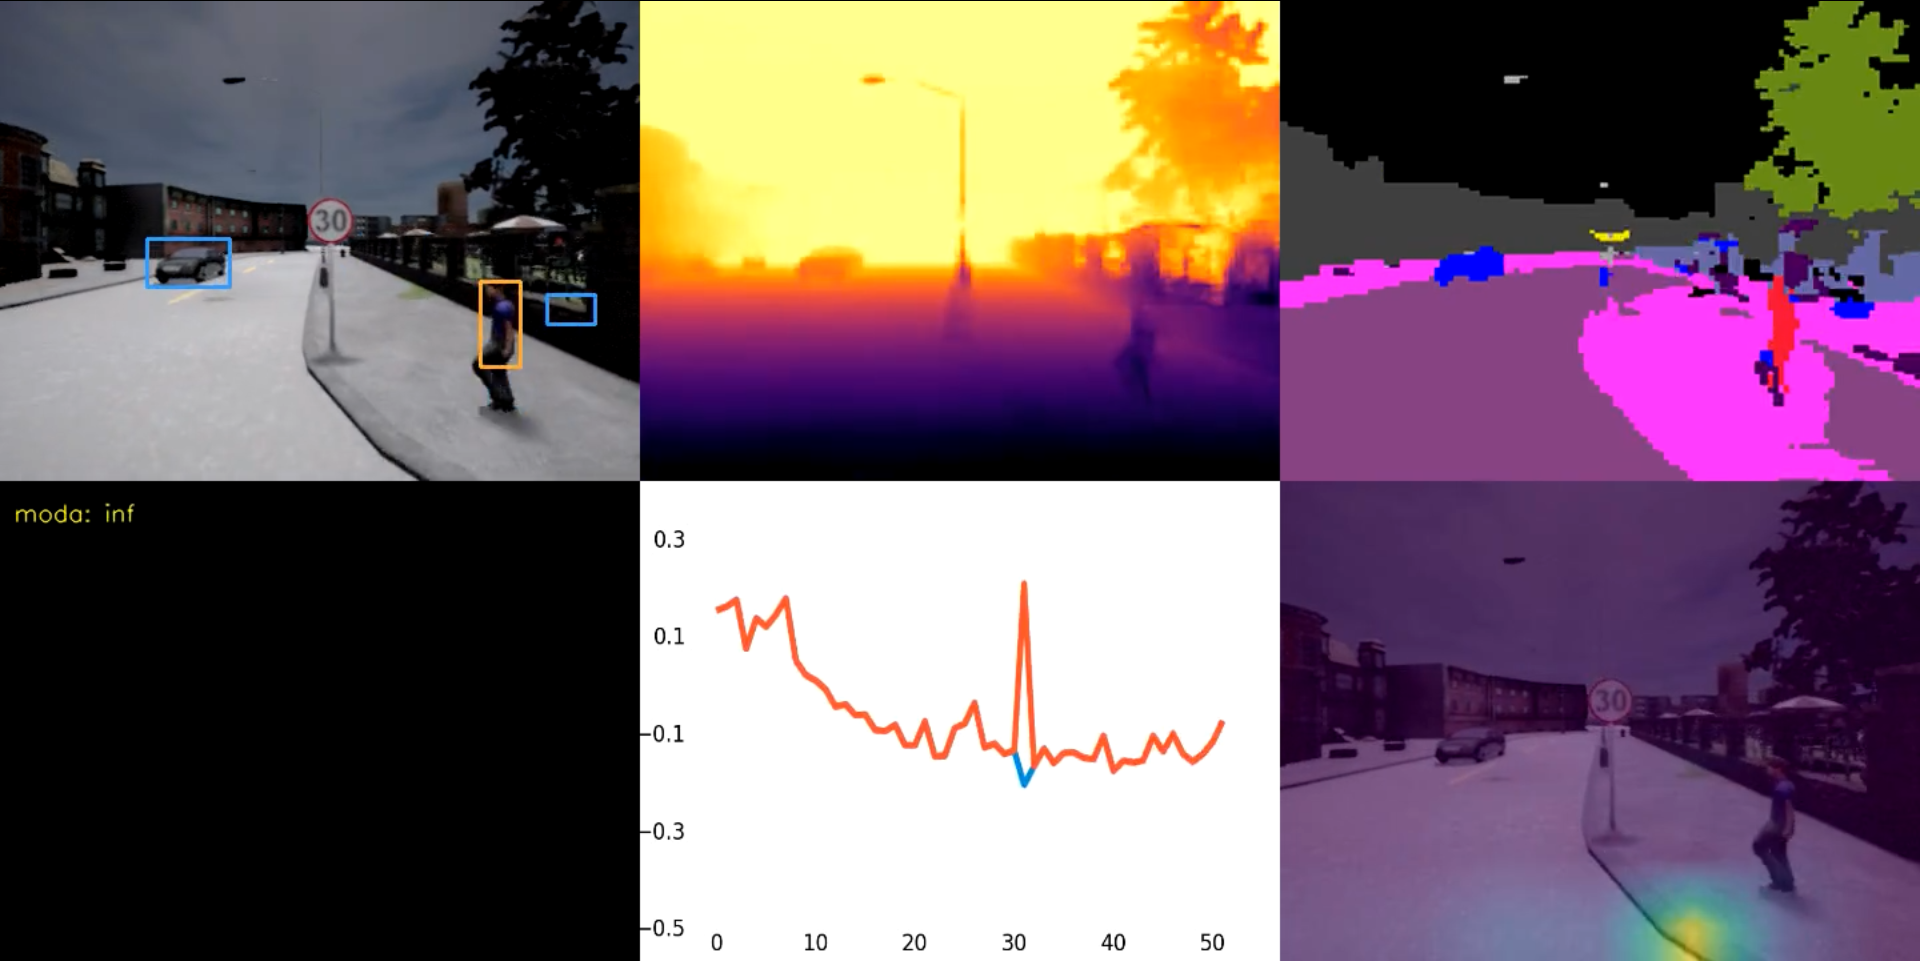
\includegraphics[scale=0.22]{imagenes/preds/crash1}
\end{figure}

\begin{figure}[H]
	\centering
	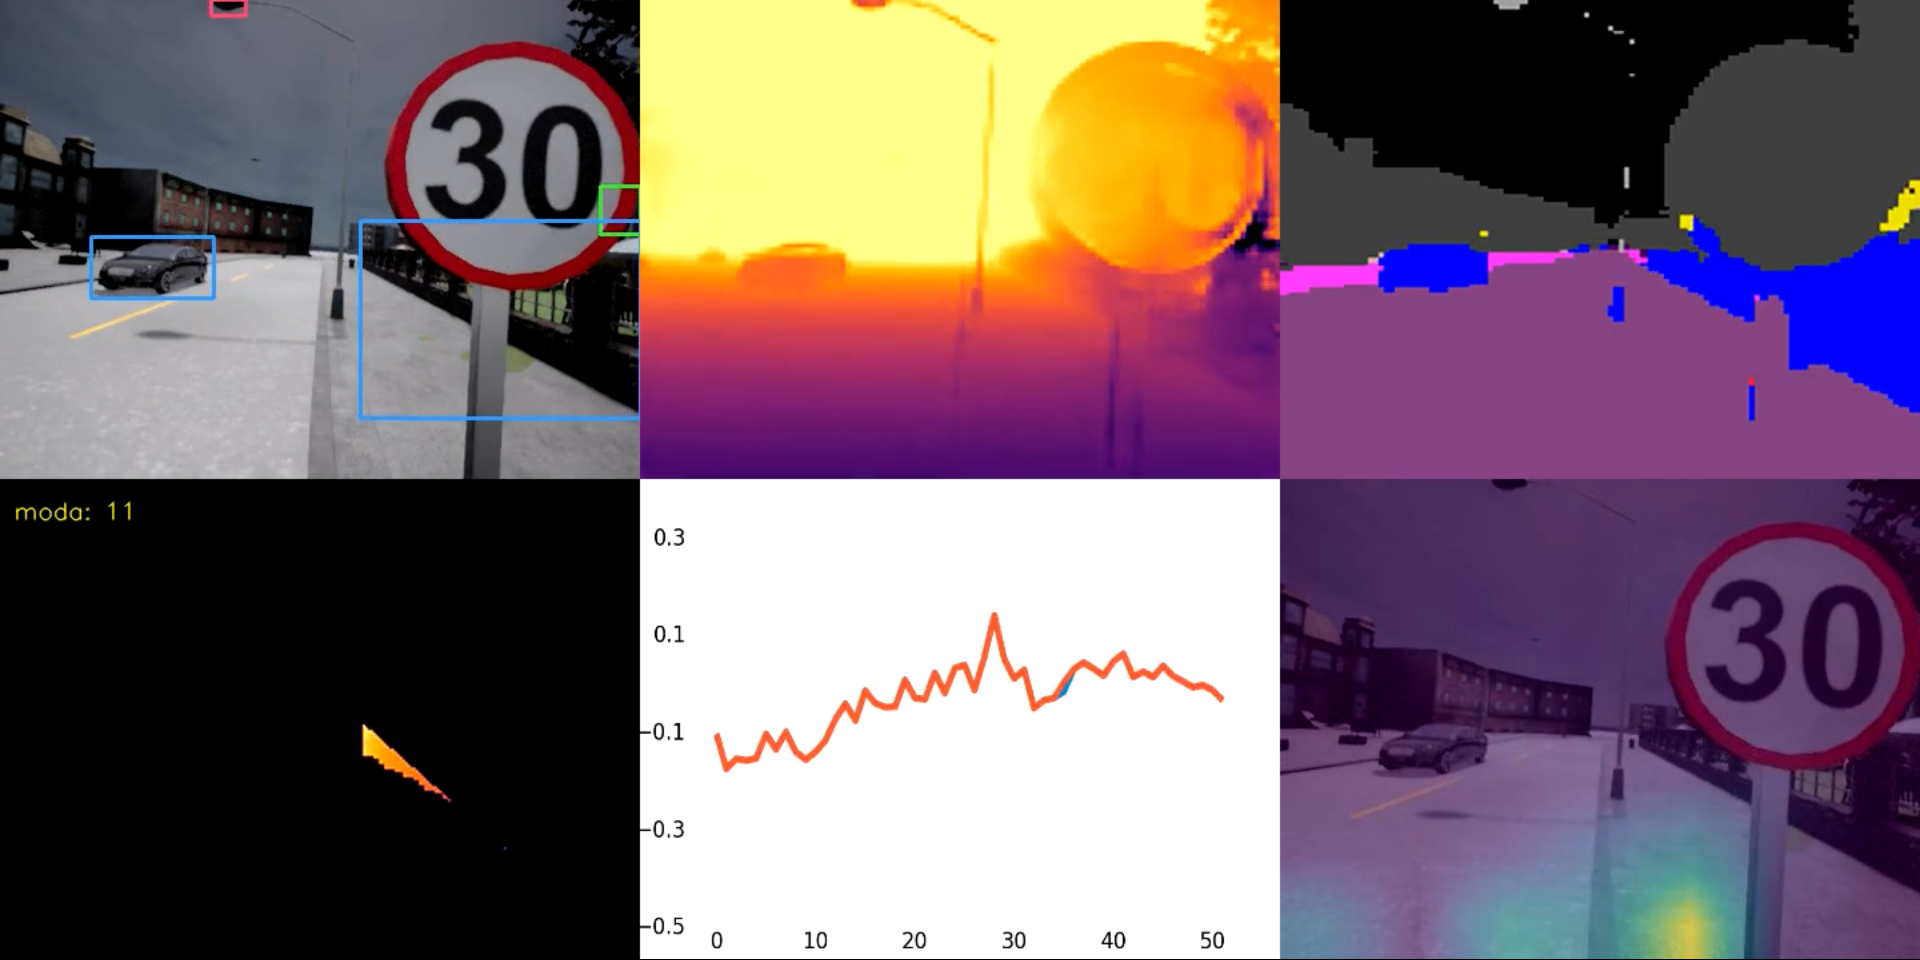
\includegraphics[scale=0.22]{imagenes/preds/crash2}
	\caption[Colisión con Poste]{colisión con poste}
	\label{colision}
\end{figure}

En total se realizaron 17 simulaciones de prueba de las cuales en 3 se cometieron errores, los cuales fueron confundir un charco como vehículo, frenando totalmente y no reanudando la marcha,  el de salirse del camino sin detectar un poste, colisionando así contra él, y el de invadir un carril en contra ruta frenando para no colisionar y congestionando el tráfico ya que no puede dar marcha atrás.
	
	\section{PRUEBA DE LA HIPÓTESIS}
	
	Para la prueba de la hipótesis ``\textit{El modelo de conducción autónoma mediante el uso de aprendizaje profundo y algoritmos de visión computacional alcanza una autonomía de nivel 2 en vías de doble sentido con separación física.}'' se siguió los siguientes pasos.
	
	\begin{enumerate}[nosep]
		\item Se evaluaron los porcentajes de exactitud de predicción de las máscaras de segmentación y estimación de distancias a partir de las salidas de la DepthNet y SemsegNet (modelos de aprendizaje profundo).
		\item Se calculó el error de detección y clasificación del color de semáforos, aplicando Flood Fill para la detección de la caja delimitadora y K-Means para la clasificación del color (algoritmos de visión computacional).
		\item Se evaluó el error de la predicción de aceleración y frenado, en base a las predicciones conjuntas de las tres redes neuronales (DepthNet, SemsegNet y DriveNet) combinadas con la clasificación de los semáforos.
		\item Se obtuvo el error de estimación de dirección tanto a la izquierda como derecha en base a la predicción de la DriveNet.
	\end{enumerate}
	
	En base a los cálculos obtenidos se puede afirmar que:
	
	\begin{itemize}[nosep]
		\item Con un porcentaje de exactitud de clasificación para la detección de obstáculos y semáforos de un $71.41\%$, el error del control longitudinal es de $\pm 0.067$, considerando valores negativos como frenado y positivos como aceleración se obtiene un $6.7\%$ de error en el control longitudinal.
		\item El error de la dirección es de $\pm0.069$ lo que da lugar a un $6.9\%$ de error en el control lateral.
		\item De las 17 pruebas realizadas un $82\%$ son satisfactorias (3 pruebas con fallos).
	\end{itemize}

	Por lo tanto con un $93.2\%$ de confianza se puede afirmar que se obtiene una conducción autónoma de nivel 2 en el $82\%$ de las situaciones (17 pruebas).
		